\section{Background and Context}
\label{sec:intro_background}

Throughout the course of human history, horses have fulfilled crucial roles as modes of transportation, military assets, and trusted companions for leisure and sporting activities. To ensure the performance of horses, humans have recognized the need for a strong emphasis on the health, fitness, and longevity of these remarkable creatures. As a result, the assessment of their fitness has remained an essential component of horsemanship.

 The earliest recorded attempts at measuring equine capabilities date back to ancient civilizations, where horses were evaluated based on their speed and endurance \cite{ani11071859}. In ancient Greece, for instance, the Olympic Games included equestrian events that showcased the athletic prowess of both horse and rider \cite{britanica}. Over time, different cultures developed their own methods of assessing equine fitness, such as the selection of warhorses based on strength and agility during battles in medieval Europe \cite{harison}.
 
In the 19th century, advancements in technology revolutionized the assessment of horse fitness and brought about a deeper understanding of equine biomechanics. The introduction of mechanical devices, such as cameras \cite{eadweardmuybridge_1899_animals} (Figure \ref{muybridge}) and accelerometers \cite{marey}, enabled limited measurements of equine gaits and biomechanical parameters.

\begin{figure}[htbp]
\centering
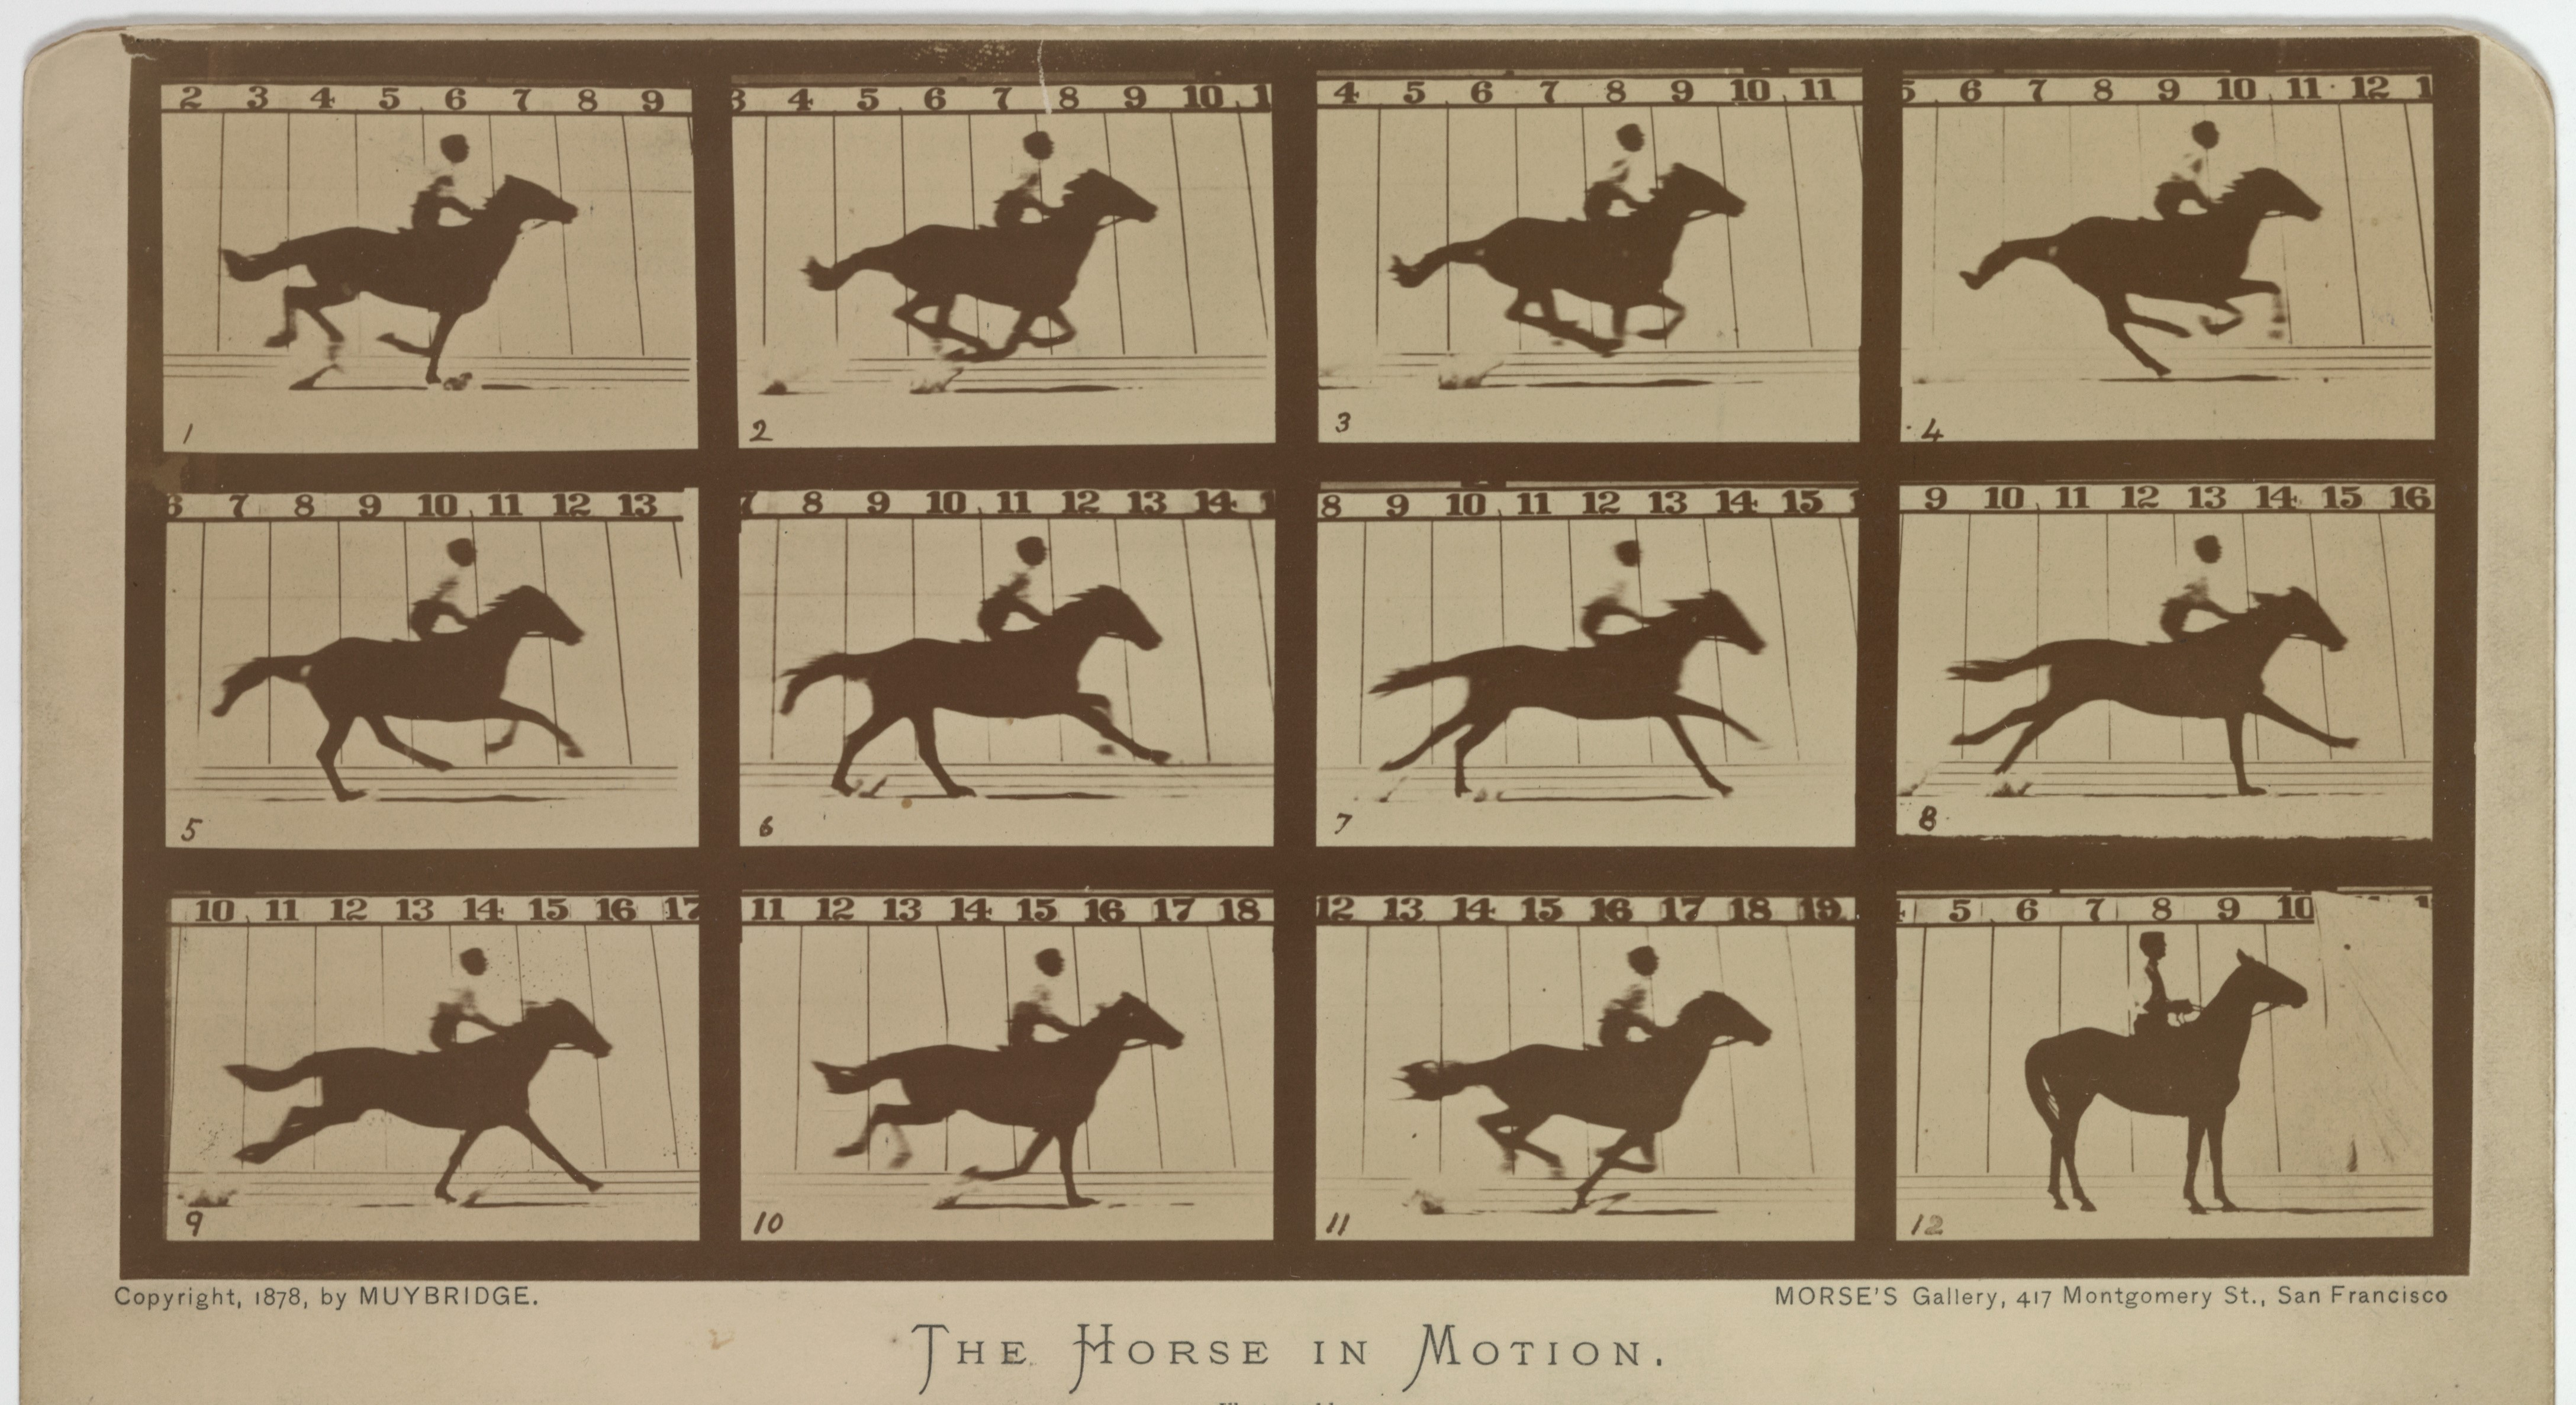
\includegraphics[width=.8\linewidth]{../tables/Muybridge.jpg}
\caption{"The horse in motion" \cite{eadweardmuybridge_1899_animals}, the first utilization of a camera for equine gait analysis.}
\label{muybridge}
\end{figure}

Measuring devices for physiological-based parameters were also invented and used in equine physiological studies. For instance, \gls{hr} and blood \gls{lac} are extensively studied parameters when evaluating athletic performance in horses. These factors serve as valuable indicators of the fatigue level and the level of effort exerted during physical activity \cite{sloet, Arfuso2021PeripheralHorses}.

Traditionally, the evaluation of fitness levels by trainers and veterinarians has relied on assessments based on observed behavior and fitness indicators like speed and stride duration. However, these assessments can be prone to errors due to inter-observer variability and the inability to capture changes over time in the animal's condition that may be indicative of impending fatigue or injury.

Fitness, in the context of both human and equine athletes, is a multifaceted concept that encompasses various physical and physiological attributes necessary for optimal performance and well-being. It involves the integration of strength, endurance, flexibility, and the efficient functioning of the cardiovascular and musculoskeletal systems. Assessing fitness accurately is crucial for developing effective training programs, preventing injuries, and enhancing overall performance.

As mentioned earlier, the training intensity and fatigue levels have been assessed using \gls{hr} and \gls{lac} measurements. As shown in Figure \ref{invasive}, measuring \gls{lac} levels is an invasive and intermittent process, as it requires multiple stops during exercise to collect blood samples. Continuous monitoring of heart rate can be achieved by equipping the horse with a heart rate monitor. Nevertheless, when considered as an individual parameter, its significance may be limited in fatigue identification, particularly in instances where emotions induce fluctuations \cite{JANSEN200938}. Therefore, the measurement of physiological parameters presents certain drawbacks, such as disrupting the training session, requiring specialized expertise, and is not feasible in all circumstances.

\begin{figure}[htbp]
\centering
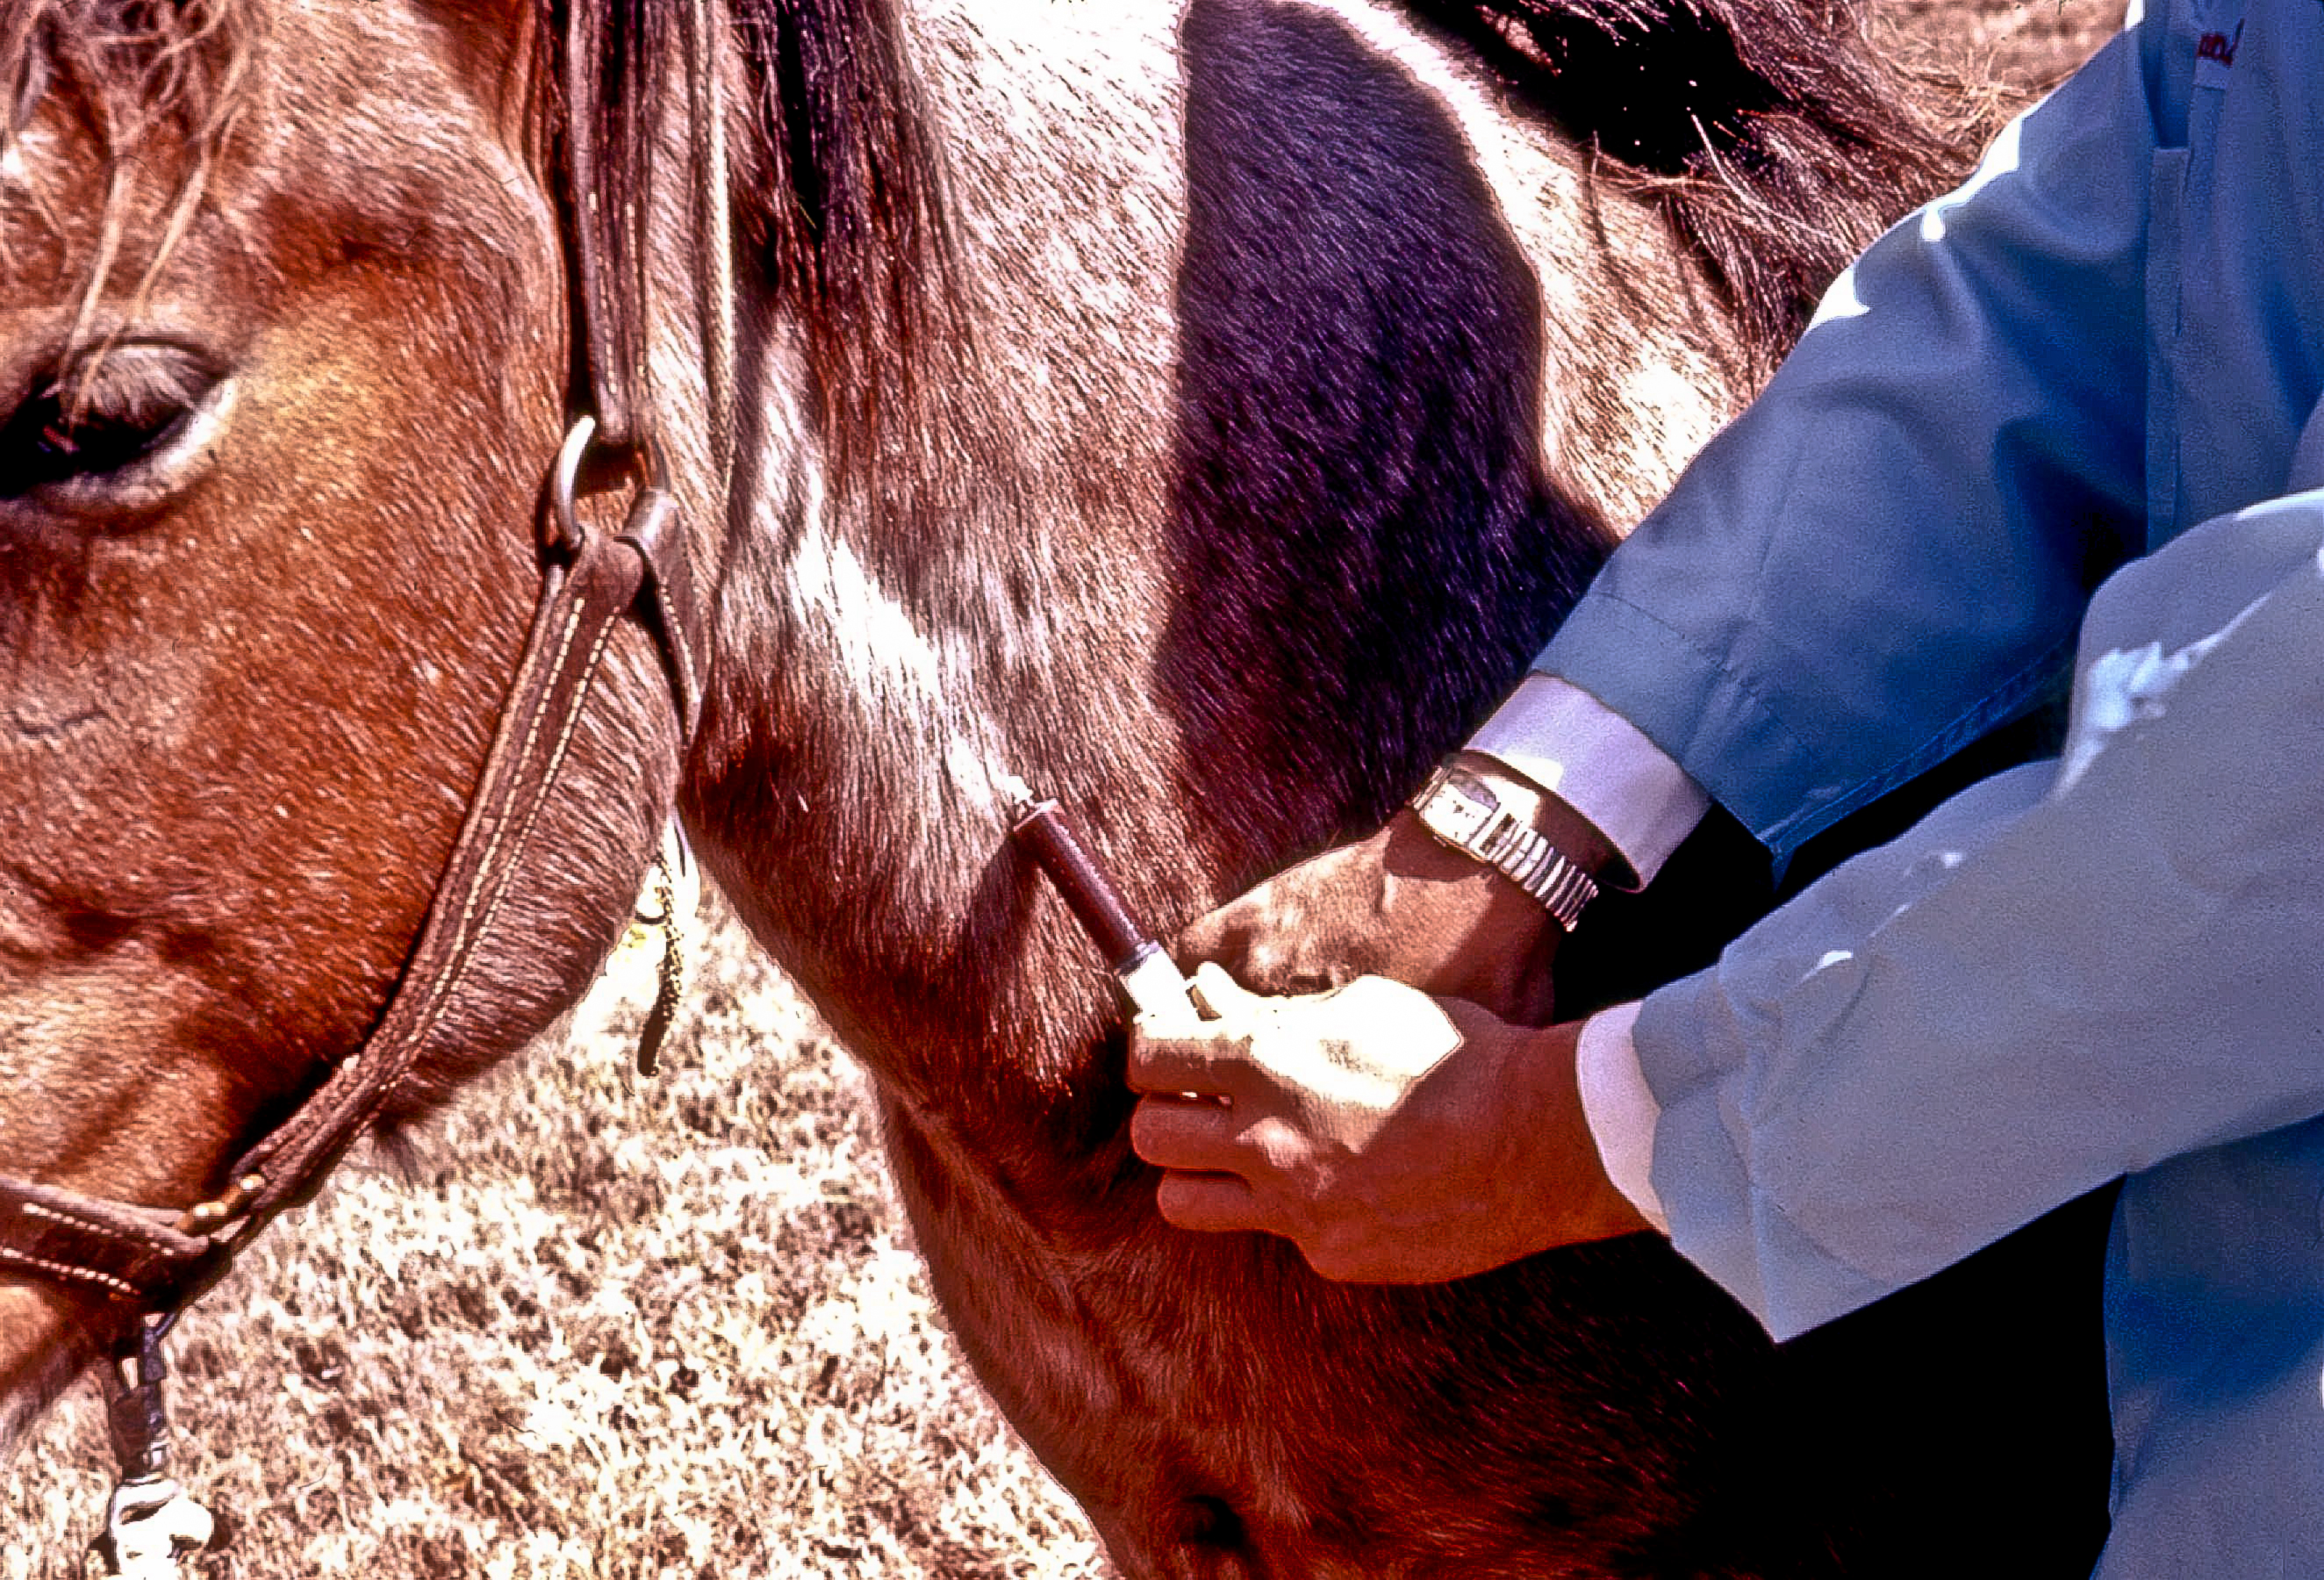
\includegraphics[width=.6\linewidth]{../tables/Blood_collection_from_horse.jpg}
\caption{Blood collection from a horse's jugular vein}
\label{invasive}
\end{figure}

In recent years, remarkable progress has been made in analyzing the gait of horses. This progress has been made possible in a precise and non-invasive manner through the utilization of measurement devices, particularly \gls{imu} sensors as wearables. These sensors have been successfully used in human sports studies to analyze and improve fitness and prevent injuries \cite{fatiguereview}. In addition, machine learning, a subfield of artificial intelligence, has emerged as a powerful tool for analyzing complex data and making predictions based on patterns hiding in the data. In recent years, machine learning algorithms have been used to tackle various problems in sport sciences, including gait analysis \cite{prakash2018} and fatigue identification \cite{lirias2803493}. Their application in the field of equine sports science is still in its infancy, but preliminary studies have shown promising results \cite{egan2018}. The combination of the data from wearable sensors and machine learning techniques holds great potential for developing methods to evaluate fitness.